\section{SNAP!}
\label{solution SNAP}
Comme expliqué précédemment, nous sommes partis d'un projet existant, SNAP BYOB, pour l'environnement de programmation. Ce projet a pour but de fournir une interface et un environnement supportant la programmation par bloc. Ce projet ne s'inscrit pas dans le cadre d'un apprentissage scolaire ou guidé. Il a donc fallu adapter le projet pour une utilisation plus scolaire. Nous allons expliquer dans cette partie les différentes adaptations que nous avons apportées au projet d'origine et pourquoi elles sont nécessaire pour remplir nos objectifs.\\

Dans les adaptations opérées, nous retiendrons : une simplification de l'interface, des fonctionnalités supplémentaires telles que la sauvegarde sur les serveurs du projet courant, une différenciation de rôle pour le professeur par rapport au public cible, une amélioration de la traduction en français, le masquage des scripts.

\subsection{L'interface}
\label{interface}
Comme expliqué précédemment le projet original n'avait pas une vocation didactique de groupe et avait un publique cible plus large que le notre. Dans cette idée, il y avait des menus pour des fonctionnalités de gestion de l'ordonnanceur et autres. Il est évident que ces fonctionnalités ne sont pas utiles pour notre public. De plus vu l'âge de notre public toutes distractions qui peuvent être évitées améliorent sensiblement la productivité de ces derniers.

Dans cette optique, nous avons opéré un nettoyage en profondeur de l'interface dans l'optique de laisser uniquement les menus utile. Toute fois comme il sera discuté dans les rôles il était intéressant de ne pas simplement les effacer, mais bien de les masquer.\\

Une autre adaptation de l'interface réalisée est l'ajout d'un menu pour les interactions avec notre plateforme web. Ce menu contient des boutons tel que : "sauvegarder sur le serveur" pour enregistrer leur travail sur la plateforme; "déscription" qui permet de retrouver le descriptif introductif de la mission; "retour à la liste des missions" qui demande à sauver le travail puis renvoi vers la page listant les missions sur le site web.

\subsection{Les rôle}
\label{role}
Dans l'optique de fournir une interface épuré pour les étudiants comme expliqué dans la section \ref{interface}. Il était nécessaire d'enlever des parties de l'interface non pertinente. Toutes foi, ces options inutiles aux étudiant peuvent l'être pour les professeurs ou dans l'optique d'avoir une missions "monde ouvert". Il est donc utile de ne pas dédoubler les interfaces mais bien d'avoir une interface modulaire suivant son utilisation. \\

Pour différencier les utilisations de l'interface, nous avons ajouté la notion de rôles. Nous avons défini deux rôle: étudiant et professeur. Grâce à cela, quand les étudiant ouvre un projet, SNAP! est lancé avec le rôle étudiant ce qui permet de ne pas affiché les options superflues. Quand c'est un professeur qui souhaite modifier une mission ou en crée une nouvelle, RSNAP lance SNAP avec le rôle professeur ce qui permet d'avoir accès au fonction avancée de SNAP.\\

Ces rôles permettent également la gestion du masquage de script. En effet il est intéressant qu'un professeur puisse masquer des blocs, mais cela ne sert à rien si les étudiants peuvent les ré-afficher.

\subsection{Masquer les scripts}
Il a été nécessaire pour la création des missions de cacher des blocs au étudiant. Par exemple la partie de vérification du code de l'étudiant ou encore le code de l'environnement de la mission ne doivent pas apparaître pour les étudiants. 

Un possibilité de cacher des blocs existait déjà dans à partie gauche de l'interface pour que tout les bloc n'apparaissent pas comme on peut le voir sur la figure \ref{fig:cacher}. Nous avons étendu cette fonction pour pouvoir également cacher des blocs ou des scripts dans la partie d'édition.

Il a également fallu ajouter cette information dans la sauvegarde du projet. Ceci a été réalisé grâce a la balise \texttt{hidden} dans le XML. Cette balise n'est présente que si le bloc doit être caché pour limiter les ajouts au document de sauvegarde.
\begin{figure}[ht]
  \begin{center}
    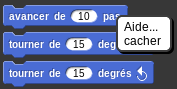
\includegraphics[scale=0.5]{content/7-solution/2-snap/images/cacher}
    \caption{Option pour cacher la définition d'un bloc}
    \label{fig:cacher}
  \end{center}
\end{figure}

\subsection{Traduction}
Le caractère francophone de ce travail est une part importante dans sa différenciation par rapport au autre initiative similaire introduit dans la section \ref{travail associé}. L'application était déjà traduite partiellement en français mais une large majorité des traduction étaient incomplètes, inexistante ou erronée. Un travail a donc été fait pour finir et amélioré la traduction de l'application, dans l'application et dans les aides.

Cette partie à été proposé au projet original de SNAP! et a été accepté chaleureusement. Ceci a 

\subsection{Fonctionnalités supplémentaires}
Comme nous avons interfacé l'application de programmation avec un site web, nous avons du reimplementer certaine fonctionnalité d'import-export.\\

Nous avions besoin de pouvoir passer le projet à l'ouverture de l'application. Pour cela, la majorité des fonctions était déjà présente. La technique utiliser était de passer l'XML contenant le projet dans la barre d'adresse du navigateur. Quelques adaptations on permis de masquer le passage du projet a l'utilisateur.\\

Dans les fonctions d'export, il y avait ici aussi des solutions existantes, mais encore une fois, n'étant pas la priorité des personnes maintenant le projet, ces fonctions étaient peu pratiques. Lors d'un export de projet, le fichier XML généré était généré dans une nouvelle page HTML. Ces fonctions ont été adaptées pour permettre de généré un XML et de l'envoyer à une adresse spécifiée.


